\documentclass[12pt,journal,compsoc]{IEEEtran}
\usepackage[cmex10]{amsmath}
\usepackage{hyperref}
\usepackage{graphicx}
\hyphenation{op-tical net-works semi-conduc-tor}


\begin{document}
\title{Genomic Fourier Power Spectra Software Filter Designs and Characteristic Learning}
\author{Micah~Thornton,~\IEEEmembership{Student Member,~IEEE,}
        and~Monnie~McGee,~\IEEEmembership{Member,~ASA,}% 
\IEEEcompsocitemizethanks{\IEEEcompsocthanksitem M. Thornton is with the Lyda Hill Department
of Bioinformatics, University of Texas Southwestern, Dallas,
TX, 75390.\protect\\
E-mail: \url{mailto:mathornton@smu.edu}
\IEEEcompsocthanksitem M. McGee is with the Department of Statistical Science at Southern Methodist University, Dallas, TX, 75206.\protect\\
E-mail: \url{mailto:mmcgee@smu.edu}}% 
\thanks{Manuscript received June 10, 2021}}%; revised July ??, 2021}}

\markboth{Eighth Biomedical Circuits and Systems Conference,~October~2021}%
{Thornton \MakeLowercase{\textit{et al.}}: Fourier Power Spectra No-Lag Matched Filters for Genomic Sequence Differentiation}
\IEEEtitleabstractindextext{%
\begin{abstract}

\end{abstract}
\begin{IEEEkeywords}
Genomic Signal Analysis,  Genomic Power Spectra Filtering,  Genetic sequence analysis, Genomic Power Spectra Convolutional Networks, Biomolecular sequence Frequency filtering, Virus Genomic Fourier Power Spectra Filtering. 
\end{IEEEkeywords}}

\maketitle

\IEEEdisplaynontitleabstractindextext

\IEEEpeerreviewmaketitle

\section{Introduction}
\label{sec:int}

\IEEEPARstart{G}{enomic} sequences are, in essence, radix four discrete-index signals, 
and contain essential information required to instantiate and replicate organisms, or non-living matter 
such as viruses and proteins.
These sequences are radix-four as a repetitive series of four base nucleotides: adenine, cytosine, guanine, 
and thymine, in Deoxyribonucleic Acid (DNA) with thymine is replaced by uracil in Ribonucleic Acids 
(RNA) constitute the information conveyed by the signals. 
Notably this characterization considers the base form of the genomic sequences as a four-valued signal, 
some prior works have considered using the hydrophobicity of the translated amino acids in conjunction 
with spectral methods for the identification of attributes of a sequence. \cite{Shu17} 
Other works have described the Methylation and other epigenetic marker profiles using a 
in this work we consider utilization of subsets of characteristic genomic Fourier power spectra which are
produced by a few different kinds of filtering techniques. 
This work treats genomic sequences as signals, and defines procedures using 

\subsection{Prior Works}
\label{sec:pw}
The concept of taking Discrete-Time Fourier Transforms (here ``time'' refers to loci along a genomic signal) 
of genomic signals dates back to the early 1990`s.  Anastassiou provides a summary of these and other
genomic signal processing techniques \cite{Ana01}. 
Yin et al. were the first to suggest the use of Fourier coefficients, and the resultant power spectra as 
numerical summaries for distance calculations and subsequent automated phylogeny construction with 
genomic sequences \cite{yin20, yin14, yin15}.
In these works the power spectra of the coefficients were subject to an even stretching (scaling) procedure 
where power spectra of shorter sequences were extended such that all sequences were of the same length


\subsubsection{Encoding \& Transforming Genomic Sequences}
Genomic/proteomic signals when digitized are usually stored in ASCII text encoded files known as FASTA/Q 
files.  Initially this acronym stood for Fast-All, referring to the capability to store any alphabet based 
sequence, for biomolecular sequences these refered to mostly genetic and proteomic sequences \cite{Lip85}.  
Prior to their storage in FASTA files, NT sequences are presented in the organic materials within which they reside, an enormously dense and resilient storage system the likes of which our engineers have not been able to reproduce. 
Once the material has been analyzed using one of many different sequencing technologies (for a nice review of modern sequencing techniques see \cite{Met10})

\begin{figure}[h!]
\caption{Genomic Signal Flow Diagram for Mixed-Radix Power Spectra Calculation} 
\label{fig:fftflow} 
\begin{center} 
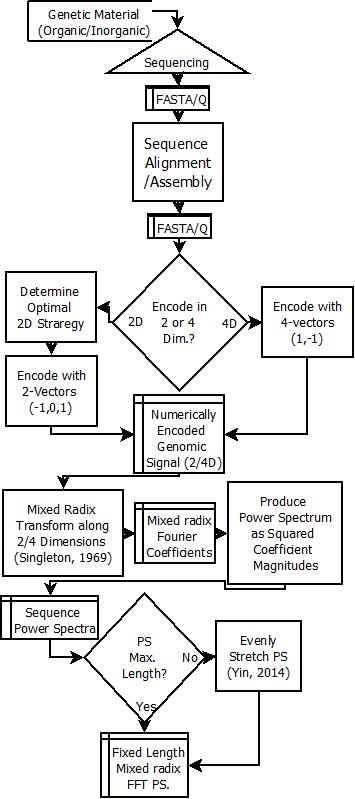
\includegraphics[scale=0.5]{Images/Files/GenomicFFTSignalFlow.png}
\end{center} 
\end{figure} 


\section{Methods \& Design}
\label{sec:meth}

The approaches discussed here seek to determine appropriate subsets of the Fourier Power Spectra 
which may be used to appropriately numerically summarize genomic signals such as DNA and RNA. 
is the application of \textit{minimal variance filtering}, the 
procedure seeks to reduce the extent of the Fourier Power Spectrum analyzed while maintaining 
relative ordering of distances among the pairs of sequences analyzed.  



\section{Results} 
\label{sec:res}

The procedures described in Section \ref{sec:meth} are applied to a sample of viral genomes
submitted by various labs during the 2020 SARS-CoV-2 pandemic curated by the GISAID Initiative \cite{gisaid}. 

Using the entire set of Fourier coefficients computed for comparison sake may not be entirely necessary, 
as a matter of fact it is possible to use a subset of just a few of the coefficients to provide roughly 
the same amount of differentiation capability. Figure \ref{fig:coeffvar} displays the variances of each 
generated set of Fourier Coefficients for the 1,397 viromes included in the study.  

\begin{figure}[h!] 
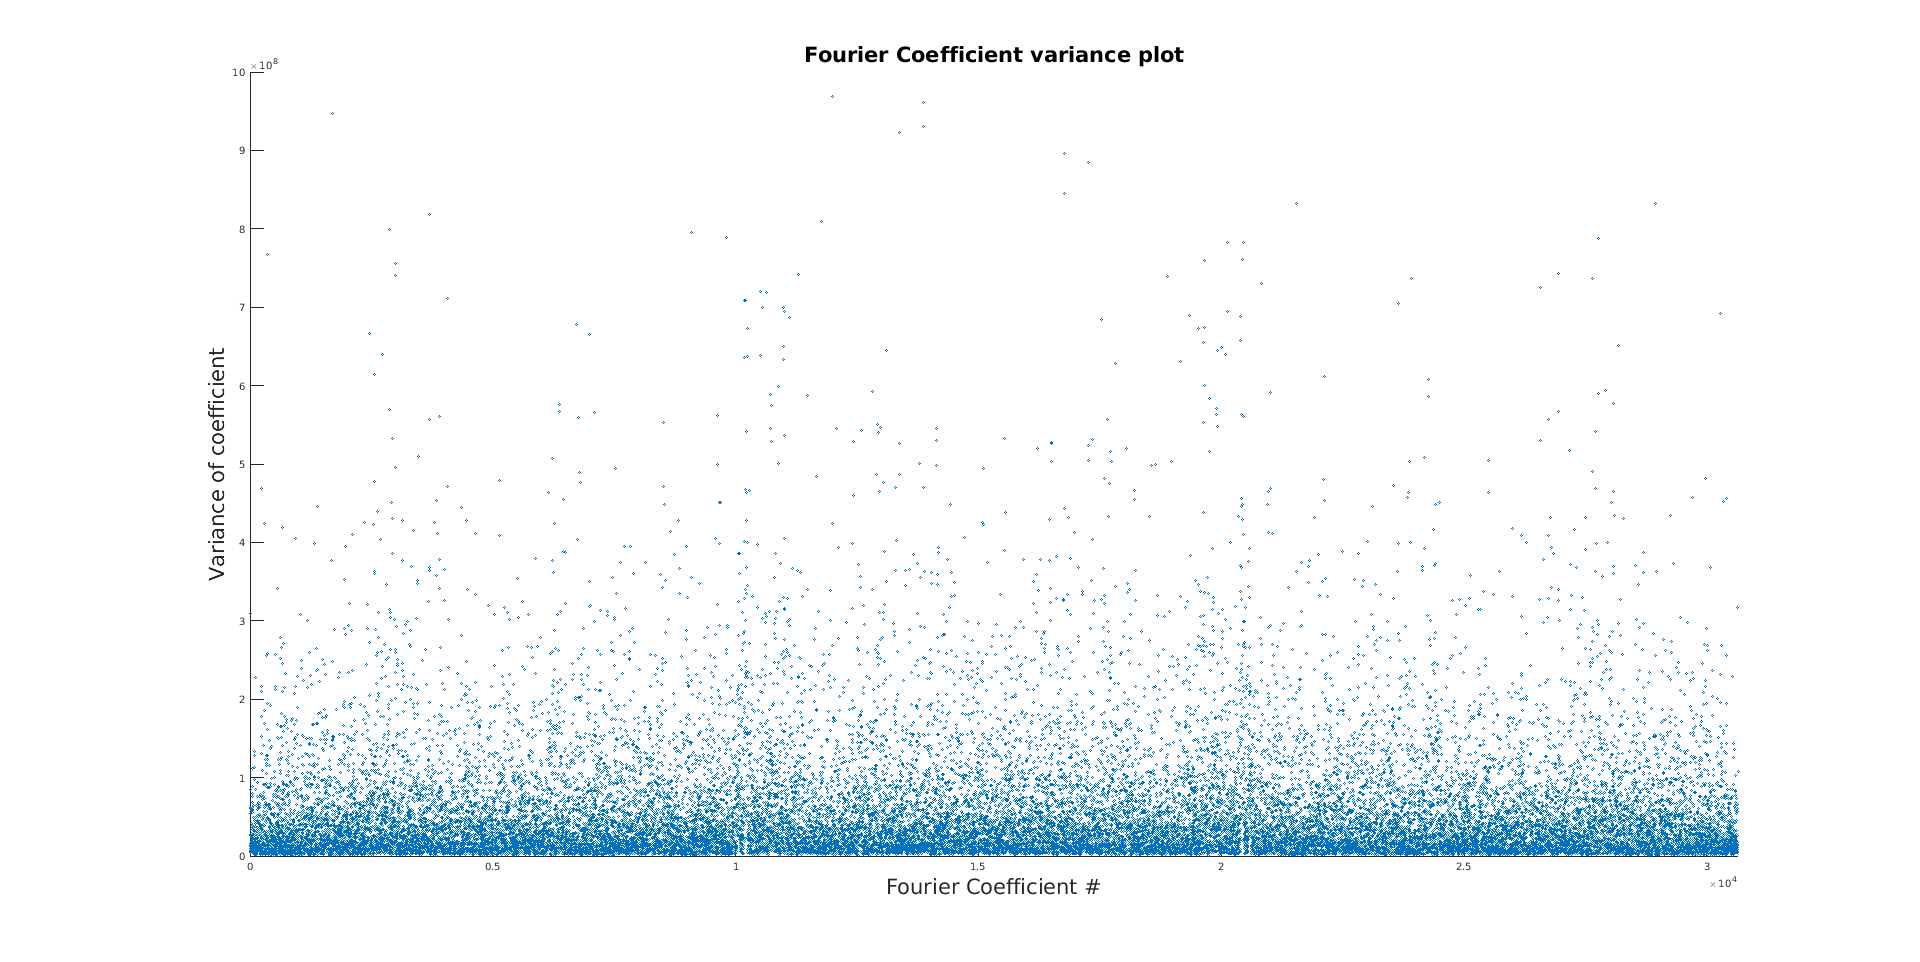
\includegraphics[width=0.5\textwidth]{Images/Files/FCoeff_var.png} 
\caption{A Plot of the Variance of each component among Viromes\label{fig:coeffvar}} 
\end{figure} 

Figure \ref{fig:coeffvar} was produced by first taking the Voss encoded Fourier coefficients that are 
computed for each of the 1,397 total viromes, scaling them each out to the maximal length, such that all 
sets of the Fourier Coefficients were of the same length, and computing the variance for each set of 
coefficients depending on their order of occurrence. On this plot, a filter applied to the coefficients may 
be selected by examining only the coefficients that have a larger variance than some threshold value. 
A histogram of some of the selected coefficients is displayed in Figure \ref{fig:coeffvarhist}. 

\begin{figure}[h!]
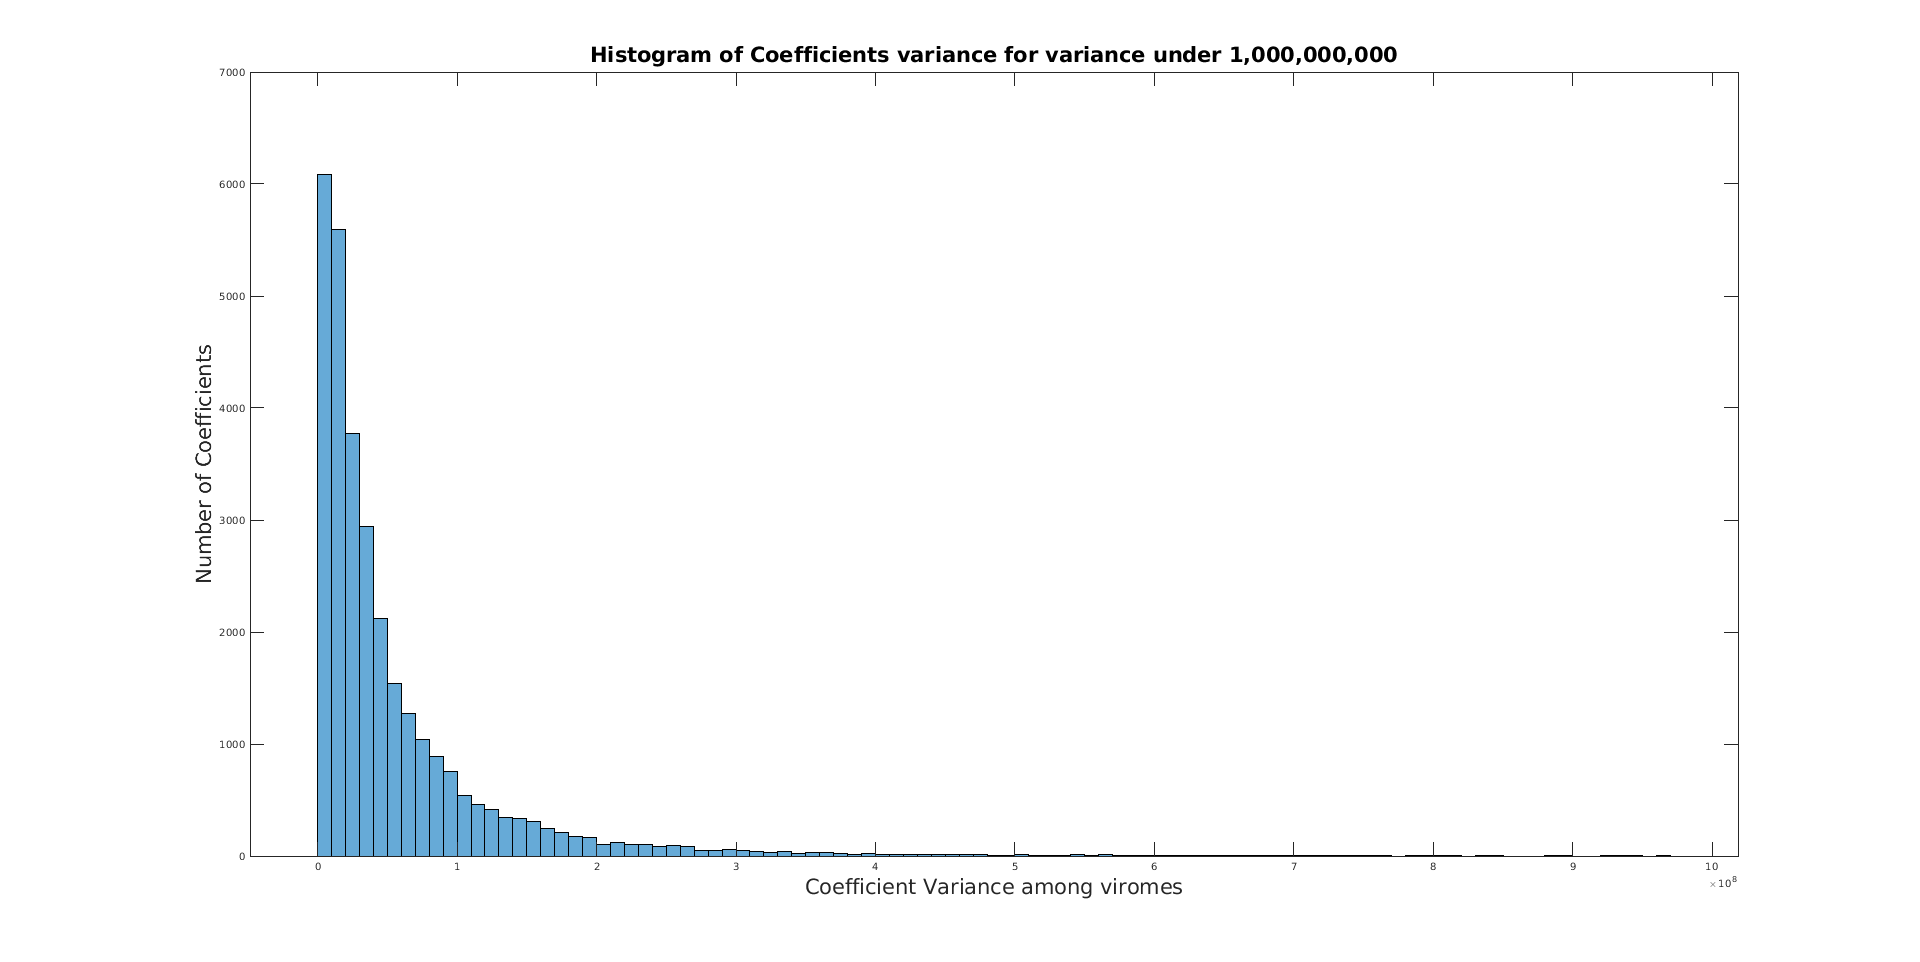
\includegraphics[width=0.5\textwidth]{Images/Files/FCoeff_var_hist.png}
\caption{Histogram of Coefficients by Variance\label{fig:coeffvarhist}}
\end{figure} 

In Figure \ref{fig:coeffvarhist} a filter may be considered as a vertical line at a given variance, beyond which the area
highlighted is the amount of coefficients that are included in the distance calculation phase.  Figure 
\ref{fig:coeffvarsurv} displays the survival curve of coefficients by their variance, that is, the
percentage of coefficients with variance greater than or equal to the ordinate is displayed as the 
abscissa. 

\begin{figure}[h!] 
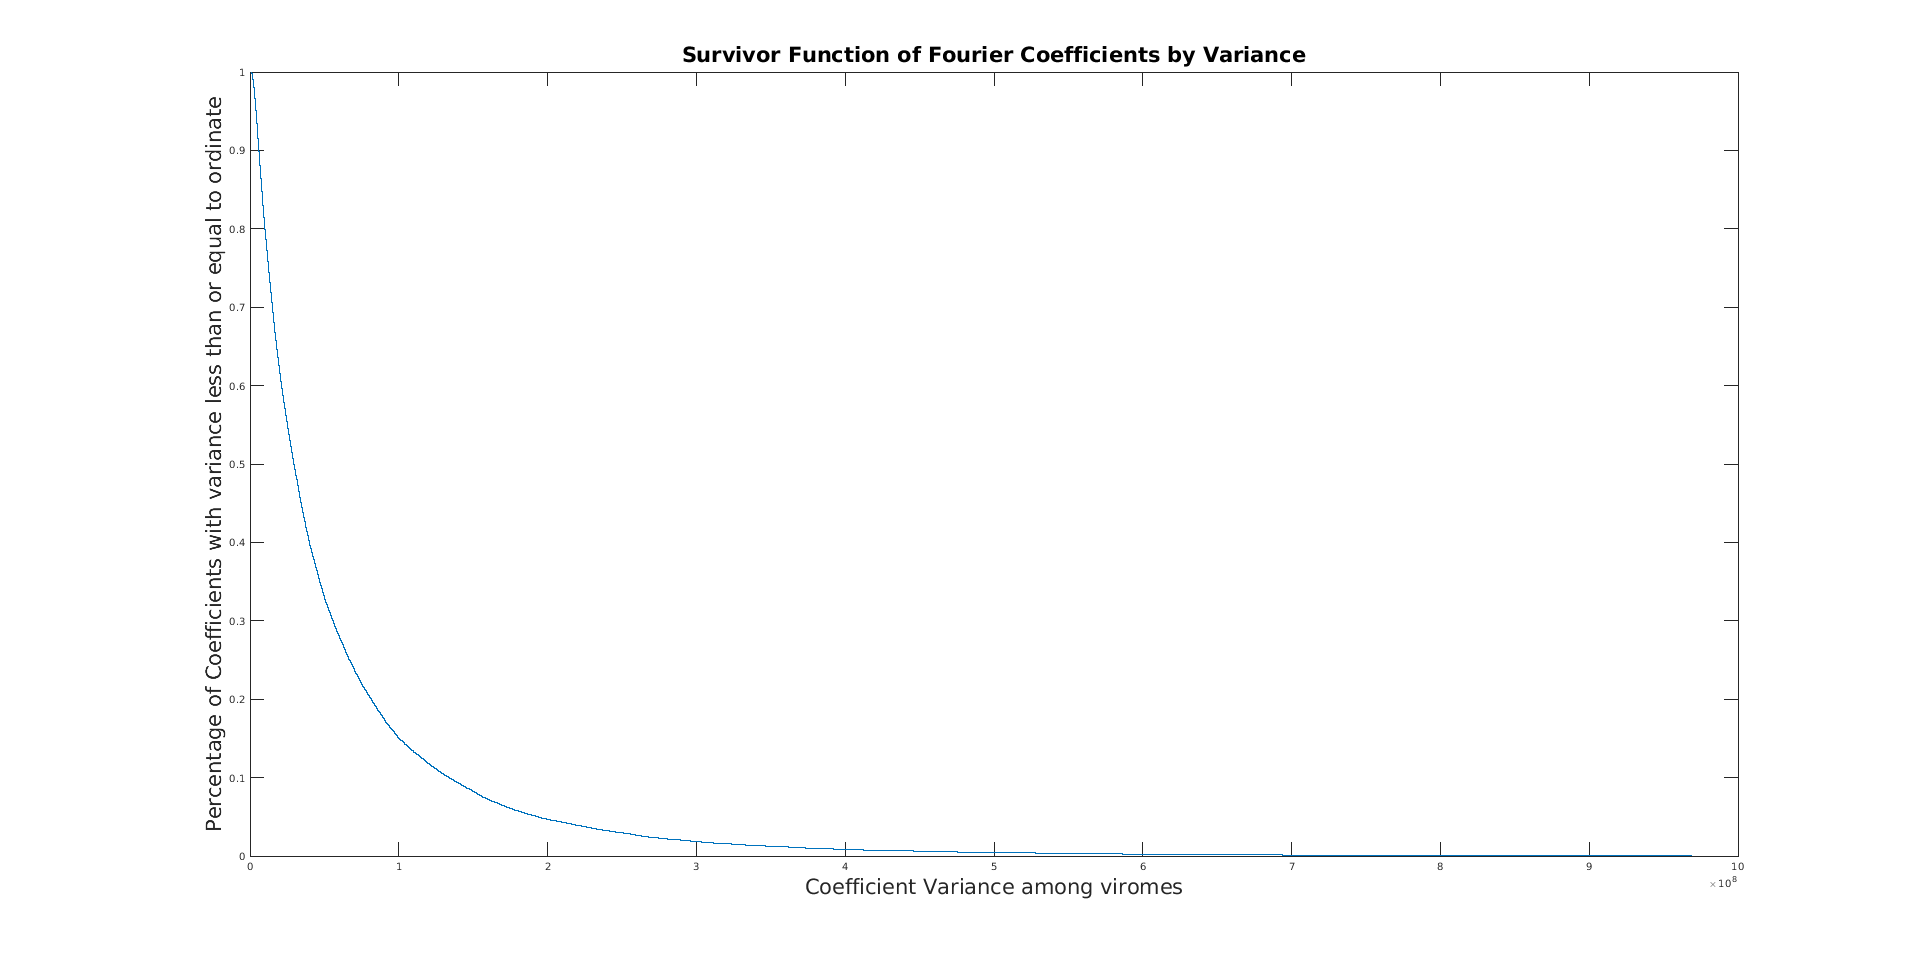
\includegraphics[width=0.5\textwidth]{Images/Files/FCoeff_var_surv.png}
\caption{Survival of Coefficients by Variance\label{fig:coeffvarsurv}}
\end{figure} 

Figure \ref{fig:coeffcorrfilt} displays the correlation of distances computed using pearson's correlation coefficient. 
The correlation is of distances computed using a subset of the coefficients of higher variance than the others, and 
displayed by the percentage of coefficients that are filtered out by variance. 

\begin{figure}[h!] 
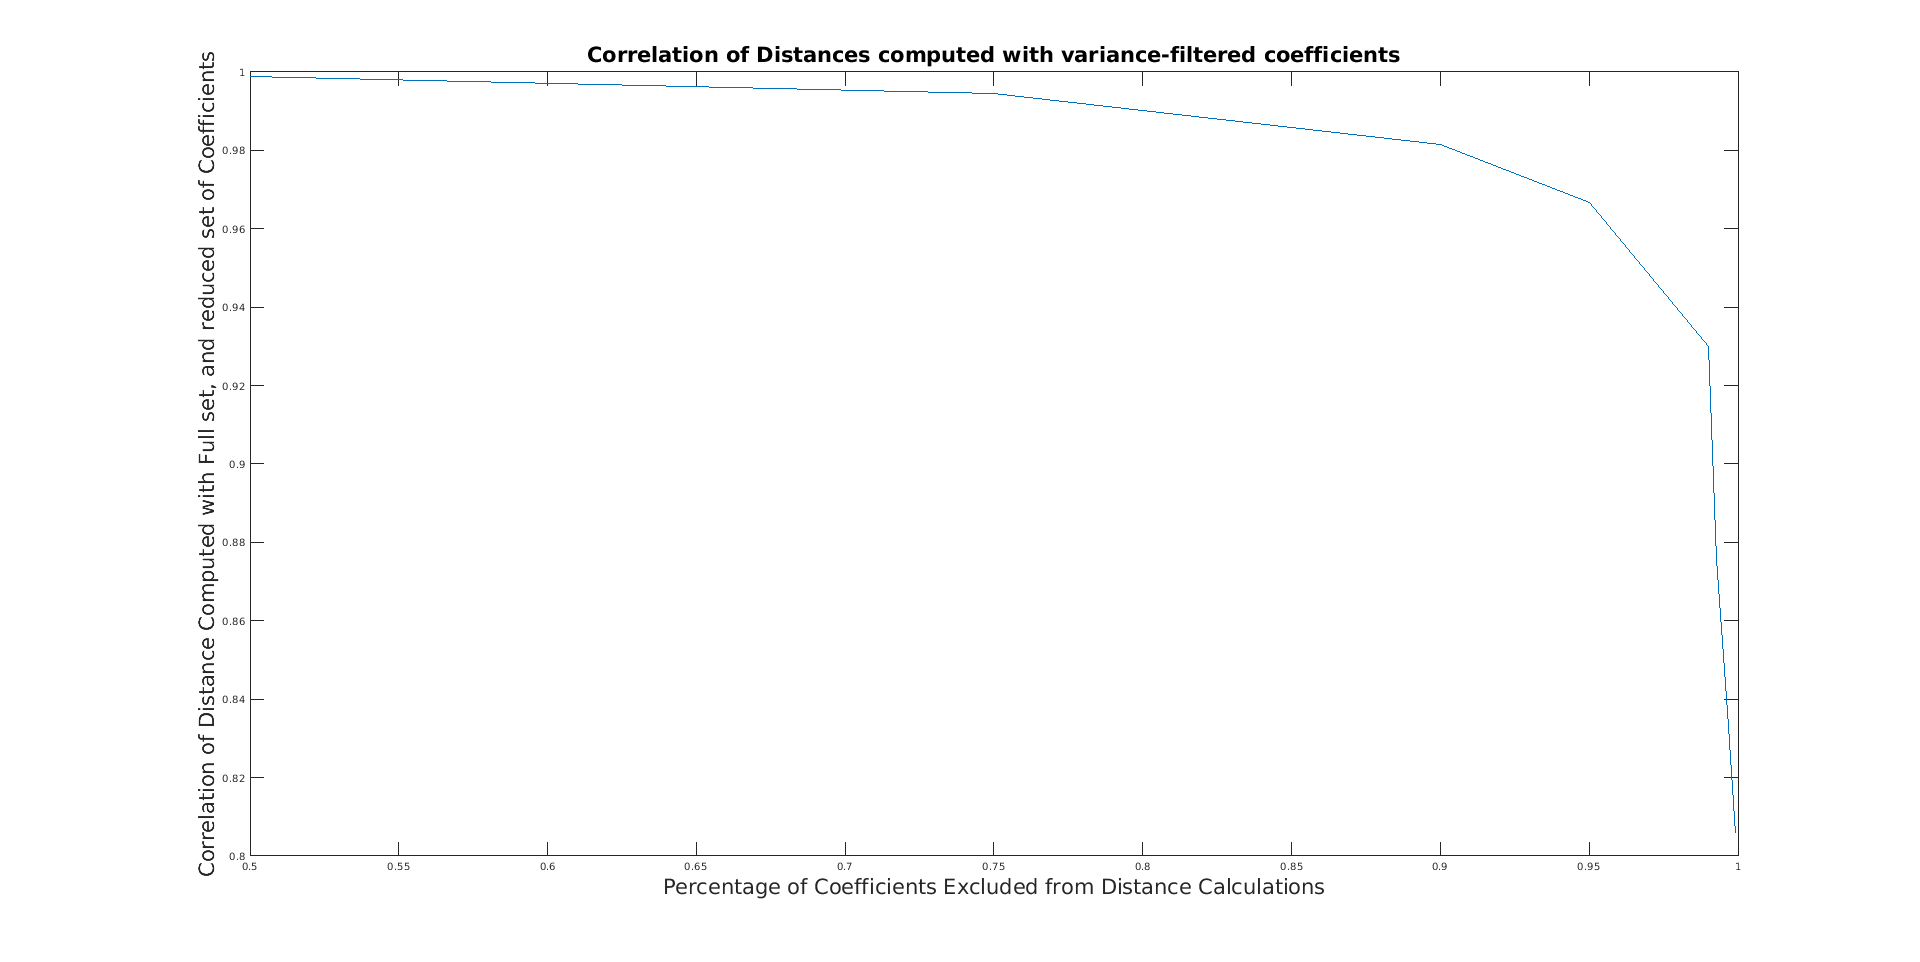
\includegraphics[width=0.5\textwidth]{Images/Files/FCoeff_Correlation_For_Filtered.png}
\caption{ Fourier Coeffients Distance Correlation to distanced computed with all coefficients\label{fig:coeffcorrfilt}} 
\end{figure} 

This filtering process may be considered as semi-analagous to that of a \textit{matched filter} from 
traditional signals processing in the following way.  As a matched filter seeks to exploit a template 
known or suspected, so too does the maximal variance filtering technique discussed here, in that once 
a threshold determination is made then each of the coefficient sequences (for the 1,394 viromes) are
matched to the template determined from the composite variances of the coefficients by selecting only 
those coefficients for which the overall variance was beyond a given threshold to complete the 
Euclidean distances calculation portion of the procedure.  The variance filtering technique does not 
however inspect the composite variances at various lagged values within the sequences, and this is 
where the analogy breaks down.  However, the procedure could accurately be considered akin to the 
\textit{matched filtering} procedure, where only the composite variance at lag zero is used. 

The plot in Figure \ref{fig:coeffcorrfilt} displays the trade-off between filtering more coefficients 
and reflection of distances as they would be computed using the full set of coefficients.  The overall 
distances computed using the coefficients are heavily influenced by the maximum variance coefficient. 
The effect is pronounced to the point that including only this coefficient in the distance calculation 
accounts for 83\% of the variation among distances observed when including all coefficients. 

This investigation reveals that only a single coefficient contains nearly as great an amount of 
information about the overall sequence as the entire set of coefficients, which would allow for 
much faster processing speeds in experiments where a large number of organisms with long sequences are 
involved.  Which leads to the next section, where a consideration of a statistical hypothesis test 
that extends from the distribution analytically described by McGee et al. in \cite{mcg98} is extended 
to test the similarity of genomic sequences. 

\section{Conclusion}
\label{sec:conc}


\appendices

\section*{Acknowledgment}

The work in this paper would not have been possible without the support of the Daehwan Kim Lab in 
the Lyda Hill Department of Bioinformatics at UTSW.  In the results section the SARS-CoV-2 viral 
genomes captured from the GISAID Initiative \cite{gisaid} reflect the combined efforts of many labs, 
for a complete listing please see \url{}.

\bibliographystyle{IEEEtrans}
\bibliography{2021BioCASRef}

\section{Acronym Dictionary} 
{\small
\begin{itemize} 
\item \textbf{ASCII} - American Standard Code for Information Interchange
\item \textbf{DFT} - Discrete Time Fourier Transform (Usually Discrete Loci, Mixed-Radix Transform)
\item \textbf{DNA} - Deoxyribonucleic Acids (Genetic Material stored in Eukaryotic Nuclei)
\item \textbf{FASTA/Q} - Fast-All File format (Q - Quality Scores)
\item \textbf{FFT} - Fast Fourier Transform (Usually Mixed Radix)
\item \textbf{GISAID} - Global Initiative on Sharing All Influenza Data (Initiative curating SARS-CoV-2 Genomes)
\item \textbf{NT(s)} - Nucleotide(s) (referring arbitrarily to Adenine, Cytosine, Guanine, and Thymine (or Uracil))
\item \textbf{PS} - Power Spectra (Usually Mixed-Radix Fourier Power Spectra)
\item \textbf{RNA} - Ribonucelic Acids (Genetic Material transcribed from DNA, existing outside Nuclei)
\item \textbf{SARS-CoV-2} - Sudden Acute Respiratory Syndrome Coronavirus 2 (Virus responsible for 2019- Pandemic)
\item \textbf{SMU} - Southern Methodist University (University in Dallas Texas) 
\item \textbf{UTSW} - University of Texas Southwestern (Medical Center \& University in Dallas, Texas
\end{itemize} 
}

\begin{IEEEbiographynophoto}{Micah Thornton}
Is a fourth year Ph.D. candidate in a joint Southern Methodist University (SMU) and University of Texas Southwestern (UTSW) Biostatistics Program.  Micah holds a Bachelor's of Science (B.S) in Computer Engineering, a B.S. in Statistical Science, and a Master's of Science (M.S) in Computer Engineering from SMU. 
\end{IEEEbiographynophoto}

\begin{IEEEbiographynophoto}{Monnie McGee} 
Is an associate professor in the Department of Statistical Science at SMU. Monnie holds a Bachelor's of Arts (B.A) in Mathematics and English from Austin College, and a Master's of Arts and Doctor of Philosophy in Statistics from Rice University.  

\end{IEEEbiographynophoto}

\end{document}


